\documentclass[a4paper, 12pt]{article}
\usepackage{listings}
\usepackage[portuges]{babel}
\usepackage[utf8]{inputenc}
\usepackage{amsmath}
\usepackage{indentfirst}
\usepackage{graphicx}
\usepackage{multicol,lipsum}
\usepackage{float}
\usepackage[export]{adjustbox}
\usepackage{matlab-prettifier}

\usepackage{geometry}
 \geometry{
 a4paper,
 total={170mm,257mm},
 left=20mm,
 top=20mm,
 }

\begin{document}
%\maketitle

\begin{titlepage}
	\begin{center}
	
	%\begin{figure}[!ht]
	%\centering
	%\includegraphics[width=2cm]{c:/ufba.jpg}
	%\end{figure}

		\Huge{UTFPR}\\
		\large{Engenharia de Computação}\\ 
		\large{Controle Digital}\\ 
		\vspace{15pt}
        \vspace{95pt}
        \textbf{\LARGE{Projeto 1: Root Locus }}\\
		%\title{{\large{Título}}}
		\vspace{3,5cm}
	\end{center}
	
	\begin{flushleft}
		\begin{tabbing}
			  Aluno: Deivid da Silva Galvão RA: 2408740\\
                Aluno: João Vitor Levorato De Souza
R.A: 2419890

\\
                Aluno: João Vitor N. Yoshida RA: 2419904\\
                Aluno: Thiago Berto Minson, RA: 2270412\\
			Professor orientador: Adalberto Zanatta Neder Lazarini \\
			%Professor co-orientador: \\
	\end{tabbing}
 \end{flushleft}
	\vspace{1cm}
	
	\begin{center}
		\vspace{\fill}
			 Novembro\\
		 2024
			\end{center}
\end{titlepage}
%%%%%%%%%%%%%%%%%%%%%%%%%%%%%%%%%%%%%%%%%%%%%%%%%%%%%%%%%%%

% % % % % % % % %FOLHA DE ROSTO % % % % % % % % % %

\begin{titlepage}
	\begin{center}
	
	%\begin{figure}[!ht]
	%\centering
	%\includegraphics[width=2cm]{c:/ufba.jpg}
	%\end{figure}

		\Huge{UTFPR}\\
		\large{Engenharia de Computação}\\ 
		\large{Controle Digital}\\ 
\vspace{15pt}
        
        \vspace{85pt}
        
		\textbf{\LARGE{Projeto 1: Root Locus}}
		\title{\large{Título}}
	%	\large{Modelo\\
     %   		Validação do modelo clássico}
			
	\end{center}
\vspace{1,5cm}
	
	\begin{flushright}

   \begin{list}{}{
      \setlength{\leftmargin}{4.5cm}
      \setlength{\rightmargin}{0cm}
      \setlength{\labelwidth}{0pt}
      \setlength{\labelsep}{\leftmargin}}

      \item Relatório do Trabalho Prático Disciplinar apresentado como requisito parcial à obtenção de nota na disciplina de Controle Digital do Curso Superior de Engenharia de Computação da Universidade Tecnológica Federal do Paraná.

      \begin{list}{}{
      \setlength{\leftmargin}{0cm}
      \setlength{\rightmargin}{0cm}
      \setlength{\labelwidth}{0pt}
      \setlength{\labelsep}{\leftmargin}}

                \item Aluno: Deivid da Silva Galvão RA: 2408740\\
               \item  Aluno: João Vitor Levorato De Souza
R.A: 2419890\\
                \item Aluno: João Vitor N. Yoshida RA: 2419904\\
                \item Aluno: Thiago Berto Minson, RA: 2270412\\
            \item Professor orientador:  Adalberto Zanatta Neder Lazarini \
      		%\item Professor co-orientador: \

      \end{list}
   \end{list}
\end{flushright}
\vspace{1cm}
\begin{center}
		\vspace{\fill}
		 Outubro\\
		 2024
			\end{center}
\end{titlepage}
\newpage
% % % % % % % % % % % % % % % % % % % % % % % % % %
\newpage
\tableofcontents
\thispagestyle{empty}

\newpage
\pagenumbering{arabic}
% % % % % % % % % % % % % % % % % % % % % % % % % % %
\section{Introdução}
    No projeto 1, vamos aplicar os conceitos aprendidos anteriormente para projetar um controlador digital para o sistema descrito pela função de transferencia contínua: 
    \begin{equation}
    \frac{s+20}{s²+1.5s+35}
    \end{equation}
    O Controlador deve atender os parametros de overshoot  $\leq$ 20\% , Tempo de subida $\leq$ 0,2s
    e Tempo de estabelecimento  $\leq$ 0,4s.
    Para alcançar esses objetivos, será realizado um estudo do comportamento dinâmico do sistema, seguido pela aplicação de técnicas de controle digital. Este processo envolve a discretização da função de transferência contínua, a seleção de um método apropriado de projeto de controlador digital, e a verificação de que o controlador atende às especificações de desempenho estabelecidas. Este relatório apresenta o desenvolvimento do controlador digital, desde a modelagem inicial até a validação final do desempenho do sistema controlado.
    
\section{Implementação}
    Pode-se observar que o sistema contínuo é estável, uma vez que seus polos estão localizados na parte negativa do plano s. Essa conclusão foi alcançada ao calcular as raízes do denominador da função de transferência, que são: -0.75 ± 5,8684i. As duas Figuras abaixo representam a saída do sistema contínuo com malha aberta, tanto para a entrada impulso quanto para a entrada degrau.

\begin{figure}[H]
    \centering
    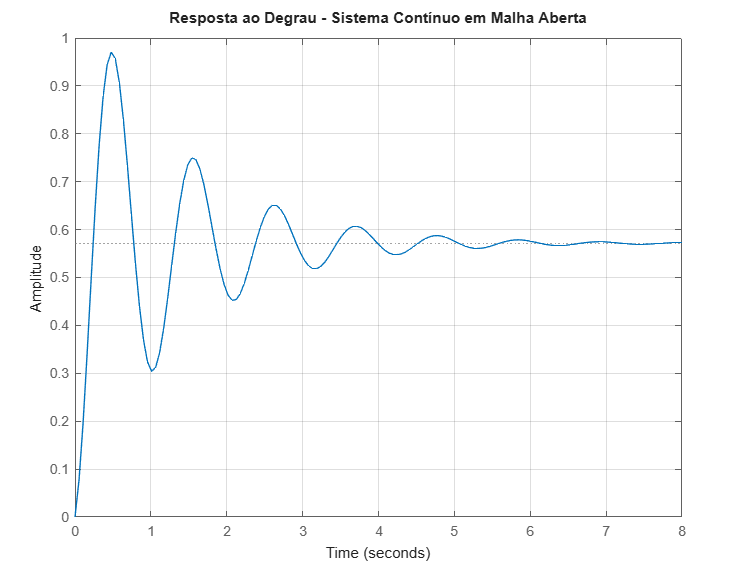
\includegraphics[width=0.9\linewidth]{qqqqq.png}
    \caption{Sistema Continuo em Malha Aberta}
    \label{fig:enter-label}
\end{figure}

\begin{figure}[H]
    \centering
    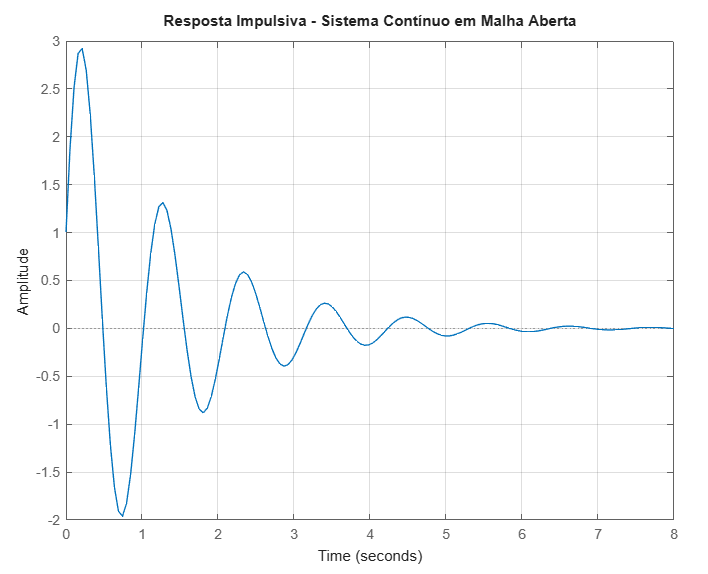
\includegraphics[width=0.9\linewidth]{99.png}
    \caption{Sistema Continuo em Malha Aberta}
    \label{fig:enter-label}
\end{figure}
\begin{lstlisting}[
frame=single,
numbers=left,
style=Matlab-Pyglike]
----------------------------------------------------
% Definir a funcao de transferencia continua do sistema
num = [1 20];
den = [1 1.5 35];
G_s = tf(num, den);
sysd=c2d(G_s,0.01)
rlocus(sysd)
rltool(sysd)
----------------------------------------------------
\end{lstlisting}

    Inicialmente foi feito a conversão do sistema continuo para um sistema discreto, onde por meio do rlocus e rltool verificamos que o tempo de amostragem de 0,1 que foi escolhido , não era possivel "juntar" os polos no rltool, portanto usamos uma frequência maior com o tempo de amostragem de 0,01.

    Foi calculado o wn e \(\xi\) a partir das especificações dos projeto
    \begin{equation}
    Ts = \frac{2,4}{Wn} \rightarrow 0.2 = \frac{2,4}{Wn} \rightarrow Wn \geq 12
    \end{equation}

    \begin{equation}
    Te = \frac{4,6}{\xi Wn} \rightarrow 0.4 = \frac{4,6}{\xi 12} \rightarrow \xi \geq 0,9383
    \end{equation}
    
\begin{figure}[H]
    \centering
    \includegraphics[width=0.8\linewidth]{aaa.png}
    \caption{Rltool}
    \label{fig:enter-label}
\end{figure}

    Os polos foram colocados em pontos 0.94 aproximadamente onde satisfaz as especificações do projeto com um overshoot próximo de 4 e o ganho obtido foi de 54,4. 
\begin{figure}[H]
    \centering
    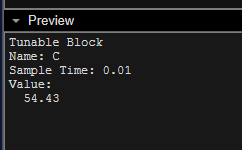
\includegraphics[width=0.5\linewidth]{DoTheL.png}
    \caption{Ganho k}
    \label{fig:enter-label}
\end{figure}

    Com o valor de ganho definido foi plotado o grafico root locus, Comparando o gráfico com os valores obtidos percebe-se que o ganho aplicado ao sistema colocou realmente as raízes nos lugares corretos.
    
\begin{figure}[H]
    \centering
    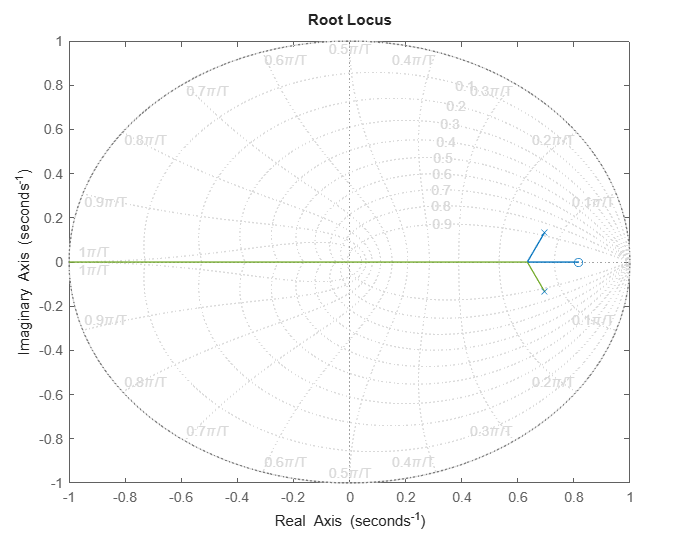
\includegraphics[width=0.9\linewidth]{MakeTheL.png}
    \caption{Rlocus}
    \label{fig:enter-label}
\end{figure}

    Em seguida, foi feita a implementação no Simulink por meio dos blocos com o intuito de representar o sistema na forma continua e discreta e poder compara-las de forma eficiente.
    
    

\begin{figure}[H]
    \centering
    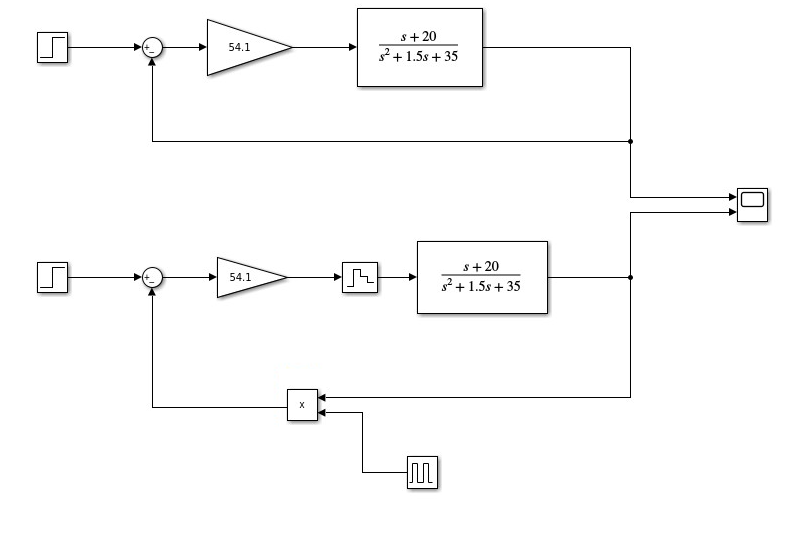
\includegraphics[width=0.87\linewidth]{asss.png}
    \caption{Diagrama de Blocos no Simulink}
    \label{fig:enter-label}
\end{figure}

    Com base nisso, foi criado um gráfico que mostra a resposta dos dois sistemas a uma entrada em degrau, utilizando um tempo de amostragem de 0,01.
\begin{figure}[H]
    \centering
    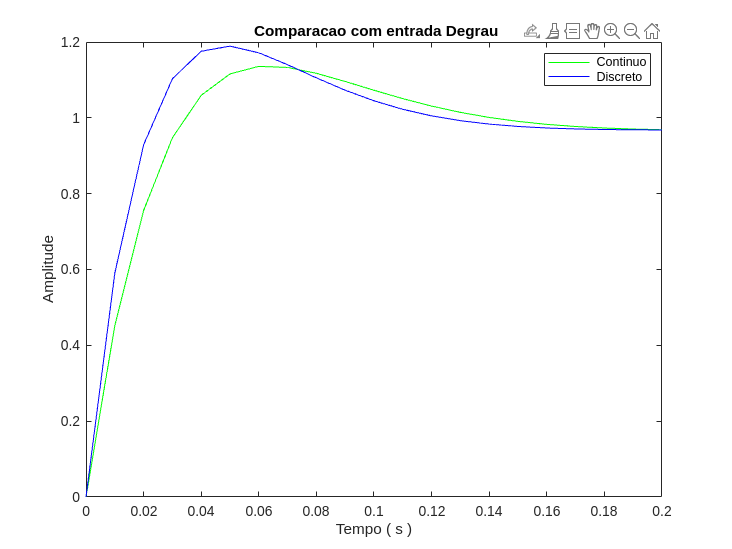
\includegraphics[width=0.9\linewidth]{777.png}
    \caption{Saída da Entrada Degrau com tempo de amostragem 0,01}
    \label{fig:enter-label}
\end{figure}

    Ao aumentar a frequência e considerar um tempo de amostragem de 0,001, observa-se uma maior aproximação do sistema contínuo.
\begin{figure}[H]
    \centering
    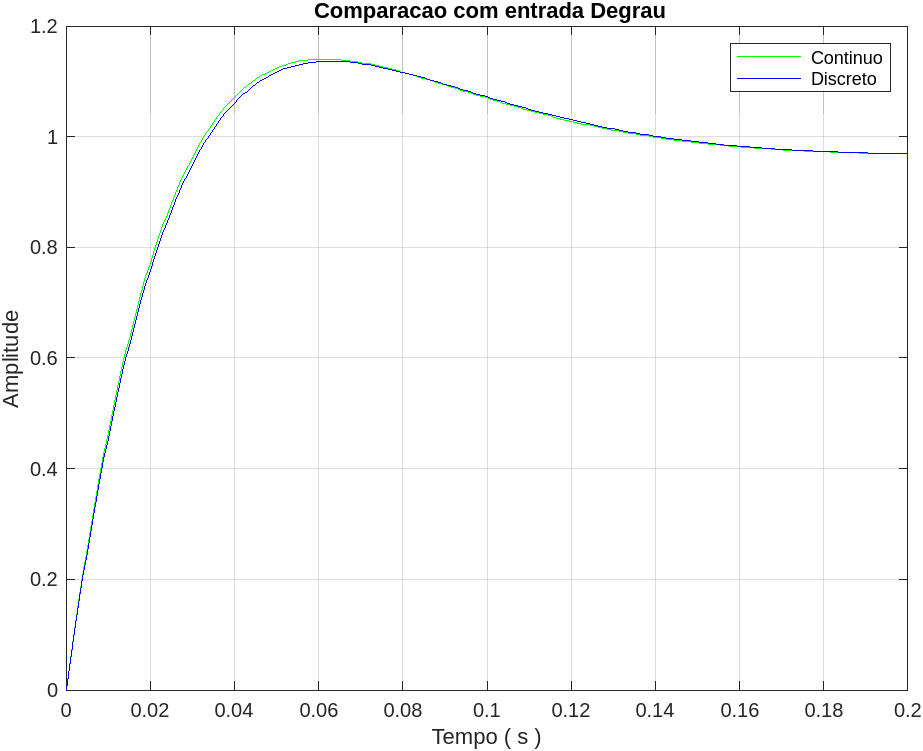
\includegraphics[width=0.9\linewidth]{CompraraDegrau2.png}
    \caption{Saída da Entrada Degrau com tempo de amostragem 0,001}
    \label{fig:enter-label}
\end{figure}

\begin{figure}[H]
    \centering
    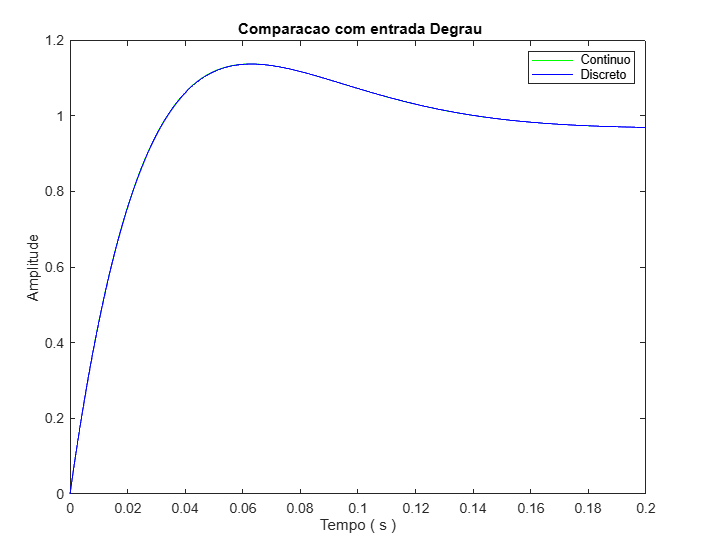
\includegraphics[width=0.9\linewidth]{wad.png}
    \caption{Saída da Entrada Degrau com tempo de amostragem 0,0001}
    \label{fig:enter-label}
\end{figure}
    Caso diminuir ainda mais o tempo de amostragem, percebe-se que fica ainda mais próximo do sistema continuo. Dessa forma, o sistema passa a emular o comportamento do sistema contínuo, assumindo suas mesmas propriedades e características.



    
\begin{lstlisting}[
frame=single,
numbers=left,
style=Matlab-Pyglike]
Ts=0.001;
% % Implementacao o ganho obtido para entrada degrau
t = 0:Ts:0.2;
sys_mf = feedback (54.4* G_s , 1) ;
sysd_mf = feedback (54.4* sysd , 1) ;
[ G_s_step , t ] = step ( sysd_mf , t ) ;
[ sysd_step , t ] = step ( sys_mf , t ) ;

% % Plotar para entrada degrau
figure
plot (t , G_s_step , 'g' , t , sysd_step, 'b') ;
title ( ' Comparacao com entrada Degrau') ;
xlabel ( ' Tempo ( s ) ') ;
ylabel ( ' Amplitude ') ;
legend ( ' Continuo ' , ' Discreto ') ;
\end{lstlisting}
\newpage


\section{Conclusão} 
Pode-se concluir que a modelagem do sistema contínuo para a forma discreta foi realizada com sucesso, atendendo a todos os requisitos especificados, onde à escolha correta do tempo de amostragem se mostrou bem importante. Com um tempo de amostragem de 0,01s, o sistema cumpre todos os requisitos, embora não seja exatamente igual ao sistema contínuo. Para obter uma semelhança total com o sistema contínuo, o tempo de amostragem deve ser de pelo menos 0,001s, permitindo que o sistema discreto emule o sistema contínuo. Por exemplo, ao aplicar uma entrada degrau com um tempo de amostragem de 0,0001s, as respostas dos dois sistemas são praticamente idênticas, tornando praticamente imperceptível a distinção entre a resposta discreta e a contínua.

\end{document}



